To enable future scientific breakthroughs and discoveries, the next generation of 
scientific applications will require extreme-scale computing performance to support the 
execution of predictive models and analysis of massive quantities of data, with 
significantly higher resolution and fidelity than what %is possible within 
can be achieved in existing 
computing infrastructure. In order to achieve the desired functional performance of 
these applications, 
%several daunting scalability challenges must be addressed. In the 
%late 90’s, terascale performance was achieved with fewer than 10,000 heavyweight 
%single-core processors. A decade later, petascale performance required about ten times as many 
%processors as terascale performance. Delivering extreme-scale computing will require one 
%million processors, each supporting 1,000 cores, resulting in a billion-core computing 
%infrastructure 
current HPC supercomputers need to increase the number of cores by orders of magnitude while also requiring a dramatic increase in the %the number of 
memory modules, communications devices and storage components~\cite{doe_ascr_exascale_2011}.
%, as depicted in Table 1. In this 
%table, the MTBF is 5 years and the checkpoint time is 20 minutes, which is estimated 
%based on a system memory of 32-64PB and an I/O bandwidth of 20-60TB/s projected in 
%the “swim-lanes”. The reported data was produced using a simulator \cite{riesen_sandia_2010}.

%\begin{table}[b!]
%	\caption{Comparison of a petascale supercomputer to an expected exascale-class supercomputer (DoE Exascale Workshop \cite{doe_ascr_exascale_2011}).}
%	\centering
%	\begin{tabular}{|c||c|cc|c|}
%		\hline
%		& & \multicolumn{2}{|c|}{Exascale (projection)} & \\
%		System Parameter & Petascale & Lane 1 & Lane 2 & Factor Change \\
%		\hline
%		System Peak & 2Pf/s & \multicolumn{2}{|c|}{1Ef/s} & 500 \\
%		Power & 6MW & \multicolumn{2}{|c|}{$\le$20MW} & 3 \\
%		System Memory & 0.3PB & \multicolumn{2}{|c|}{32-64PB} & 100-200 \\
%		Total Concurrency & 225K & 1B$\times$10 & 1B$\times$100 & 40,000-400,000 \\
%		Node Performance & 125GF & 1TF & 10TF & 8-80 \\
%		Node Concurrency & 12 & 1,000 & 10,000 & 83-830 \\
%		Network BW & 1.5GB/s & 100GB/s & 1,000GB/s & 66-660 \\
%		System Size (nodes) & 18,700  & 1,000,000 & 100,000 & 50-500 \\
%		I/O Capacity & 15PB & \multicolumn{2}{|c|}{32-64PB} & 20-67 \\
%		I/O BW & 0.2TB/s & \multicolumn{2}{|c|}{20-60TB/s} & 10-30 \\
%		\hline
%	\end{tabular}
%	\label{tbl:projection}
%\end{table}

The explosive growth in the number of components significantly exacerbates the propensity of extreme-scale 
computing systems to faults. %, while driving power consumption to unforeseen heights. 
Regardless of the individual components' reliability, system
resilience will continue to decrease as the number of components increases, as shown in Figure~\ref{fig:exe_failure}. For example, a 
system of 1 million components, each averaging a fault every 25 years, is expected to experience a 
fault every 10 minutes.

To avoid the full 
re-execution of an application upon failure, traditional fault tolerance methods periodically checkpoint
the execution state of the applications, such that recovery
can be achieved by restarting from a consistent checkpoint when failure occurs~\cite{kalaiselvi_sadhana_2000}. 
Recent works \cite{mills_2014_icnc,riesen_sandia_2010} have shown that such solutions are unlikely to scale to the level of faults 
anticipated in extreme-scale environments. Given the increase in system failure rates and the time 
required to checkpoint large-scale compute- and data-intensive applications, it is very likely
that the time spent on checkpointing and recovery
%required to periodically checkpoint an application and restart it upon failure 
may exceed the system mean time between failures \cite{riesen_sandia_2010}, %. Consequently, applications may achieve
%very little computing progress, 
thereby reducing considerably the overall performance of the
system. %Figure~\ref{fig:exe_faults} illustrates this fact and shows that, using coordinated 
%checkpointing, the system efficiency drops dramatically as the number of sockets increases. The reported data was produced using a simulator~\cite{riesen_sandia_2010}. 
Furthermore, the nature and frequency of errors in extreme-scale computing are such that
checkpoint-restart may not be an adequate approach to handle the diverse types of faults in
these environments. 
Several studies have shown the same concern and proposed process replication as a
possible solution [49, 55]. 
%Unfortunately, in so far as performance is concerned, resilience to failures and adherence to 
%power budget constraints are two conflicting objectives, as achieving high performance may push
%the system’s components past their thermal limit and increase their likelihood of failure.

Process replication, also referred to as state-machine replication, is a well-known technique that has been 
shown to scale to meet the resilience requirements of large distributed and mission-critical systems~\cite{schneider_1990_tutorial}.
Based on this technique, a process's state and computation are replicated across independent computing
nodes. When the main process fails, one of the replicas takes over the computation task. Replication 
requires at least doubling the number of computing resources, since each process must have at least 1 replica, thereby 
limiting the system efficiency to 50\%. %A consequent shortcoming of process replication in HPC is the
%increased power consumption caused by the need for additional resources to tolerate failure, which
%might exceed the power budget imposed upon extreme-scale machines.

\begin{figure}[!t]
	\begin{center}
		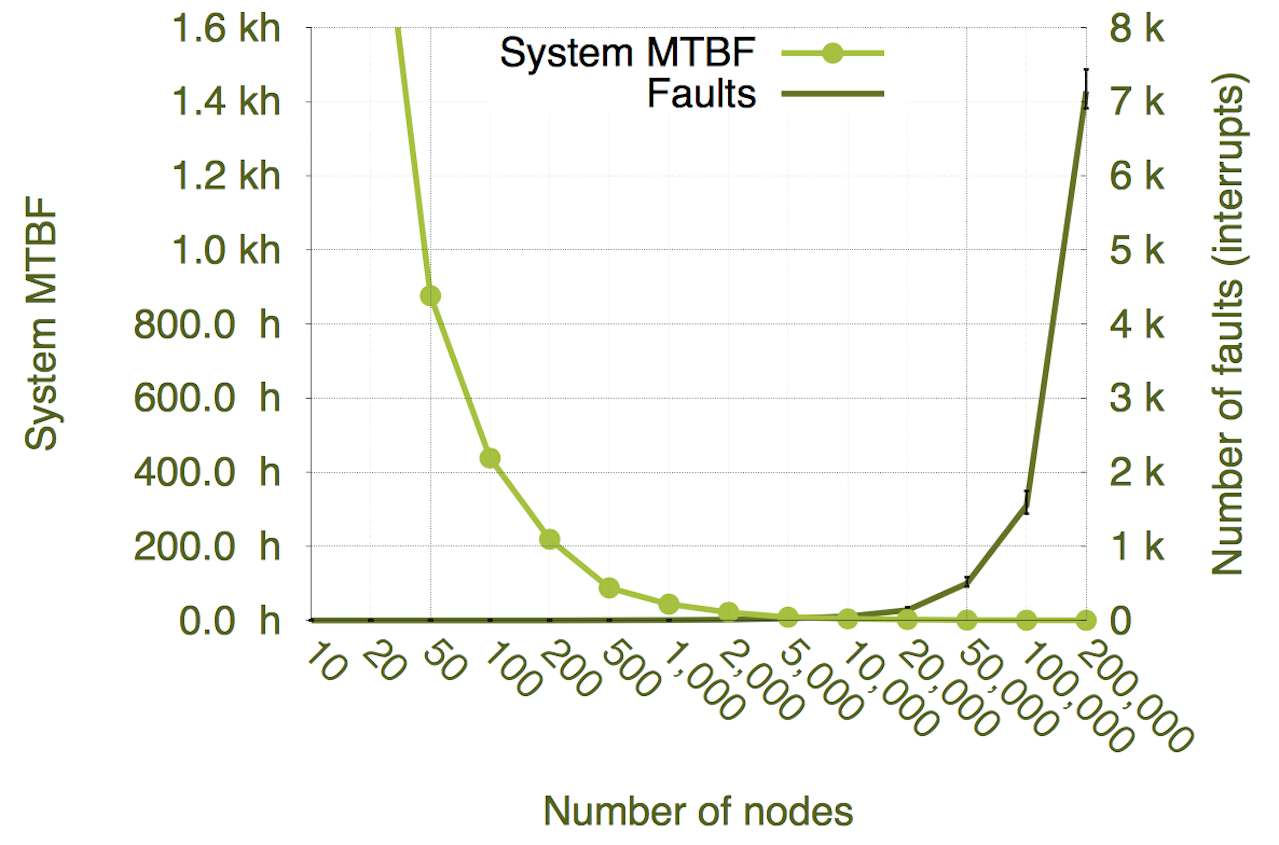
\includegraphics[width=0.9\columnwidth]{Figures/sandia_system_failure_rate_increase_nodes}
	\end{center}
	%\vskip -0.25in 
	\caption{Impact of system size on system resilience.}
	\label{fig:exe_failure}
\end{figure}

%\begin{figure*}[!t]
%	\begin{center}
%		\subfigure[System resilience projection \cite{riesen_sandia_2010}]
%		{
%			\label{fig:exe_failure}
%			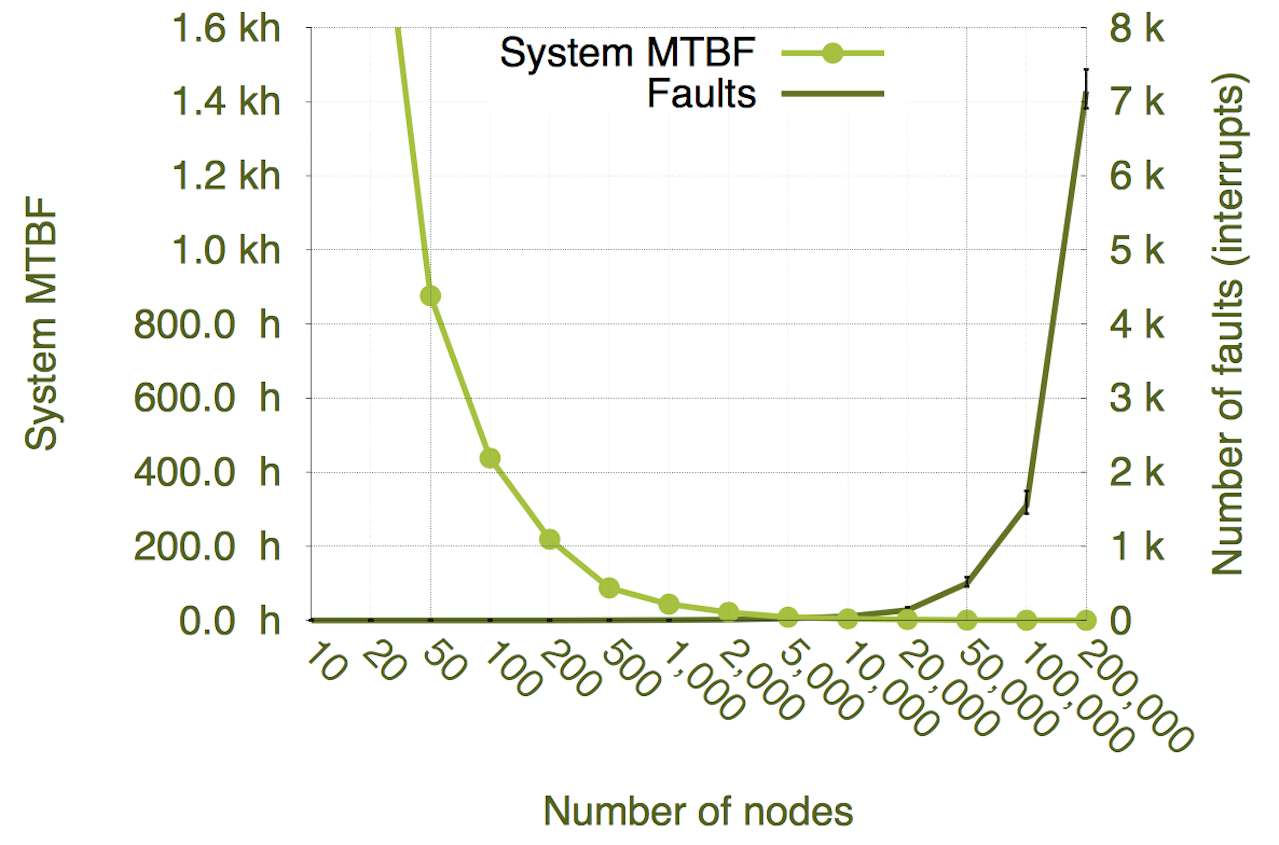
\includegraphics[width=0.3\textwidth]{Figures/sandia_system_failure_rate_increase_nodes}
%		}
%		\subfigure[System efficiency projection]
%		{
%			\label{fig:exe_faults}
%			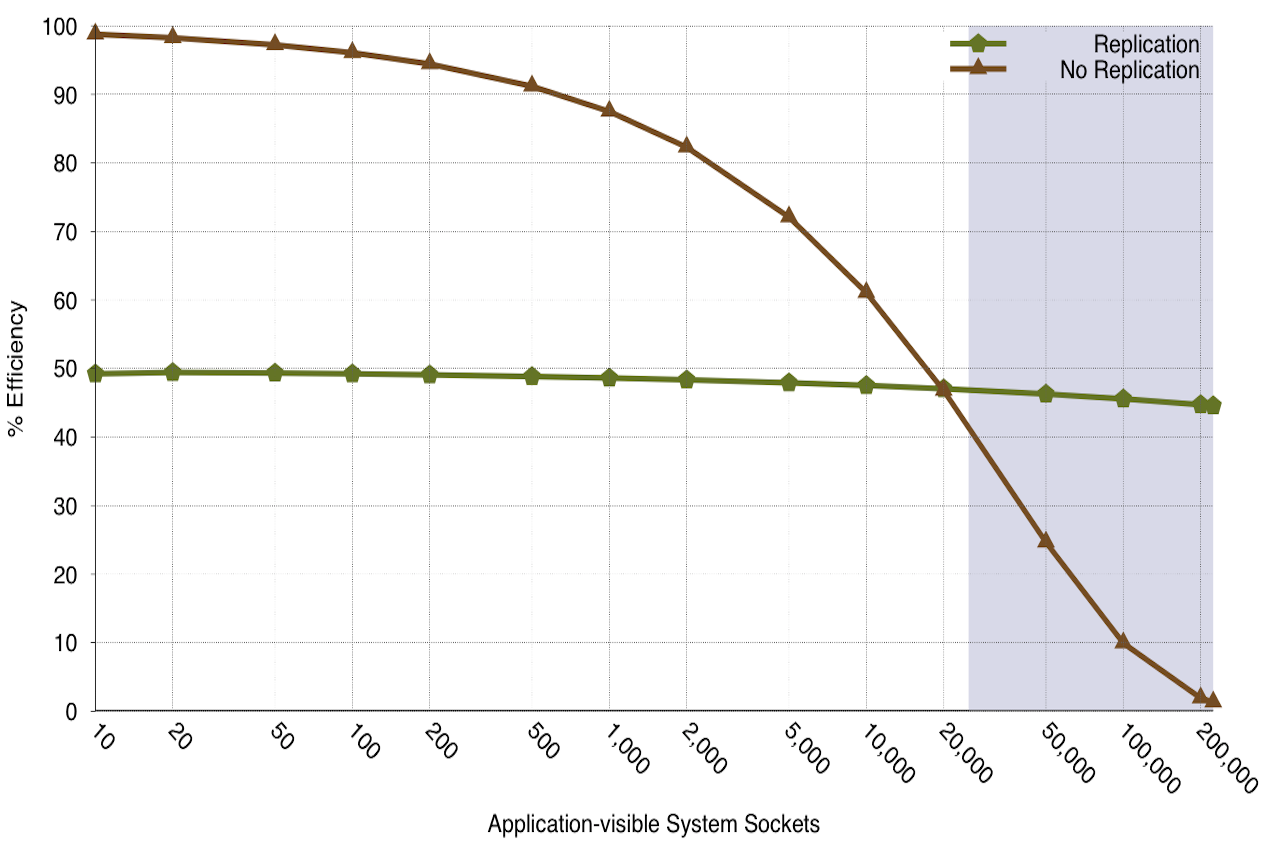
\includegraphics[width=0.3\textwidth]{Figures/faults}
%		}
%		\subfigure[System power projection \cite{sandia_exascale_projections}]
%		{
%			\label{fig:exe_power}
%			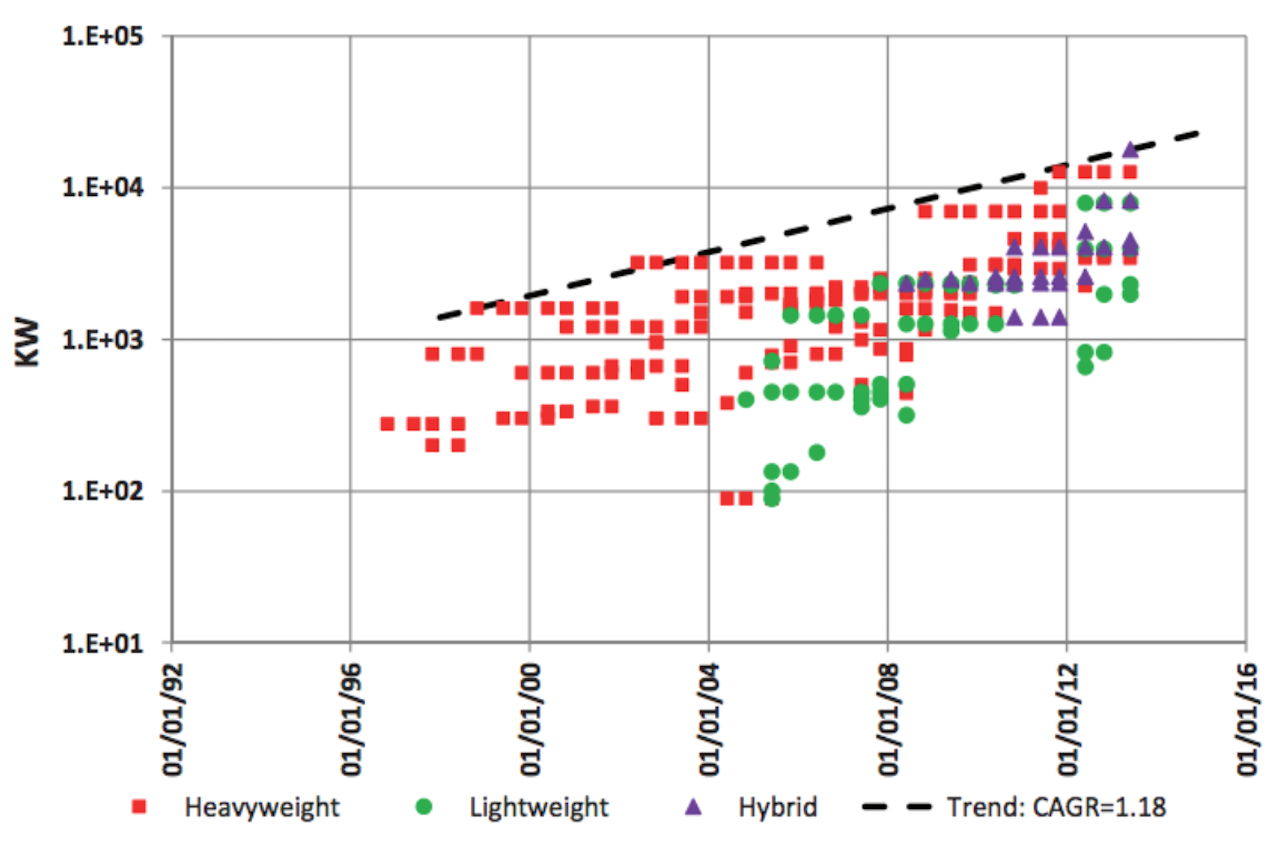
\includegraphics[width=0.3\textwidth]{Figures/power}
%		}		
%	\end{center}
%	\caption{Projections for future extreme-scale systems.}
%	\label{fig:exe_projection}
%\end{figure*}

%With the explosive growth in the number of components comes a 
Another direct consequence of the increase in system scale is the dramatic increase in
power requirements. Analysis in~\cite{doe_ascr_exascale_2011} shows a steady rise of system power consumption to 1-3MW in 
2008, followed by a sharp increase to 10-20MW in subsequent years, with the expectation that
it could surpass 50MW by 2016, making system power a leading design constraint on the path to extreme-scale computing. The US Department of Energy has recognized this trend and established a power 
limit of 20 megawatt \cite{doe_ascr_exascale_2011}, challenging the research community to provide 
a 1000x improvement in performance with only a 10x increase in power. Although largely pragmatic\footnote{The constraint is derived from an estimated cost of \$1 million
per MW per year and a power budget of \$20 million per year.}, adhering to 
%a prescribed 
this power constraint is critical to the design 
and operations of extreme-scale computing systems. The power-limits placed upon extreme-scale systems 
is at the heart of the tradeoff between power consumption and time-to-solution. Although the 
intricacies of this tradeoff are complex, operating under power-constraints is a reality that 
future extreme-scale system designers must face, making the relationship between computing performance
and power consumption increasingly more critical.


%Another direct consequence of the increase in the number of components, is the increasing 
%propensity of the system to failure. Regardless of the individual components' reliability, system
%resilience will continue to decrease as the number of components increases\footnote{For example, a 
%system of 1 million components, each averaging a fault every 25 years, is expected to experience a 
%fault every 10 minutes.}. To avoid the full 
%re-execution of a failing application, traditional fault-tolerant techniques typically checkpoint
%the execution state of the applications, periodically. Upon the occurrence of a fault, recovery
%is achieved by restarting the computation from a safe checkpoint \cite{kalaiselvi_sadhana_2000}. 
%Recent work \cite{mills_2013_e2sc,mills_2014_icnc,ferreira_sc_2011,riesen_sandia_2010,bougeret_tech_2012
%,casanova_inria_2012} have shown that existing solutions are likely not to scale to the level of faults 
%anticipated in extreme-scale environments. Given the increase in system failure rates and the time 
%required to checkpoint large-scale compute- and data-intensive applications, it is very likely
%that the time required to periodically checkpoint an application and restart it upon failure 
%may exceed the system mean time between failures \cite{riesen_sandia_2010}. Consequently, applications may achieve
%very little computing progress, thereby reducing considerably the overall performance of the
%system. Figure~\ref{fig:exe_faults} illustrates this fact and shows that, using coordinated 
%checkpointing, the system efficiency drops dramatically as the number of sockets increases. Furthermore, the nature and frequency of errors in extreme-scale computing are such that
%checkpoint-restart may not be an adequate approach to handle the diverse types of faults in
%these environments. 
%Several studies have shown this same behavior and proposed process replication as a
%possible solution [49, 55]. 


%Process replication, also referred to as state-machine replication, is a well-known technique that has been 
%shown to scale to meet the resilience requirements of large distributed and mission-critical systems.
%Based on this technique, a process's state and computation are replicated across independent computing
%nodes. When the main process fails, one of the replicas takes over the computation task. Replication 
%requires at least doubling the number of nodes, since each process must have at least 1 replica, thereby 
%limiting the system efficiency to at most 50\%. A consequent shortcoming of process replication in HPC is the
%increased power consumption caused by the need for additional resources to tolerate failure, which
%might exceed the power budget imposed upon extreme-scale machines.

Insofar as performance is concerned, resilience to failures and adherence to 
power constraints are two conflicting objectives, as achieving high performance may push
the system's components past their thermal limit and increase their likelihood of failure.
The inherent instability of extreme-scale computing systems, in terms of the envisioned high-rate and 
diversity of their faults, together with the demanding power constraints under which these systems will be
designed to operate, %makes it extreme challenging to deliver efficient extreme-scale computing. 
calls for a reconsideration of the fault tolerance problem. The main objective
of this paper is to explore novel paradigms for resilience in future extreme-scale
systems. 

To this end, we propose a proactive, power-aware resilience model, referred to as \textit{Lazy
Shadowing}, as an efficient and scalable alternative to achieve high-levels of resilience, through
forward progress, in extreme-scale, failure-prone computing environments. In the proposed
resilience model, each process is associated with a replica, which runs concurrently with its main 
process. For clarity, the original process is referred to as the main (process) and the replica as the 
shadow (process). The shadow executes the same code as its
associated main process, but at a reduced CPU rate and on a different computing node. The rate
at which the shadow runs is derived based on the expected time-to-solution of the supported
application, the power constraints imposed by the underlying computing infrastructure, and the
likelihood of failure. Upon failure of the main process, the shadow increases its 
execution rate to complete the task, thereby reducing the impact of such a failure on the progress of
the remaining tasks. Successful completion of the main process, however, results in immediate
termination of the shadow. Since the failure rate of an individual component is much lower than that of 
the whole system, it is very likely that, most of the main processes complete their execution
successfully. Consequently, the coupled execution of a main process and its associated shadow 
dramatically increases a power-constrained system's tolerance to failure, at a significantly reduced
energy consumption.

The rest of the paper is organized as follows. We begin with a survey on related work in Section 
\ref{sec:related_work}. Section \ref{sec:frame_model} defines the Lazy Shadowing 
computational model and Section \ref{frame_multiple} discusses how Lazy Shadowing can be used in 
extreme-scale computing environments for efficient fault tolerance. 
We then introduce three analytical models for performance assessment
in Section \ref{sec:analytical}, 
followed by experiments and evaluation in
section \ref{sec:evaluation}. Section \ref{sec:conclusion} concludes this work and points out 
future research directions.





















